\section{Auswertung}
\label{sec:Auswertung}
\subsection{Berechnung der Grenzfrequenzen aus der Durchlasskurve}
Zunächst wird, wie in der Durchführung beschrieben, die Spannungsamplitude am Ende der $LC$-Kette in Abhängigkeit der Frequenz betrachtet.
Der mithilfe des $XY$-Schreibers entstandene Graph ist in Abbildung \ref{fig:durchlass} dargestellt.
Auf der $y$-Achse ist die Spannungsamplitude, auf der $x$-Achse der natürliche Logarithmus der Frequenz dargestellt.
Exemplarisch wurden an der $x$-Achse mehrere Frequenzwerte eingetragen, wobei diese den realen Frequenzwert und nicht dessen Logarithmus darstellen.
Um nun die Grenzfrequenzen möglichst genau ablesen zu können, wird eine lineare Regression durchgeführt.
Diese wird für die Längeneinheiten auf der $x$-Achse und die Logarithmen der Frequenzen für die abgelesenen Werte durchgeführt.
Alle abgelesenen Werte sind wiederum nochmals in Tabelle \ref{tab:durchlass} angegeben.\\
\begin{figure}
  \centering
  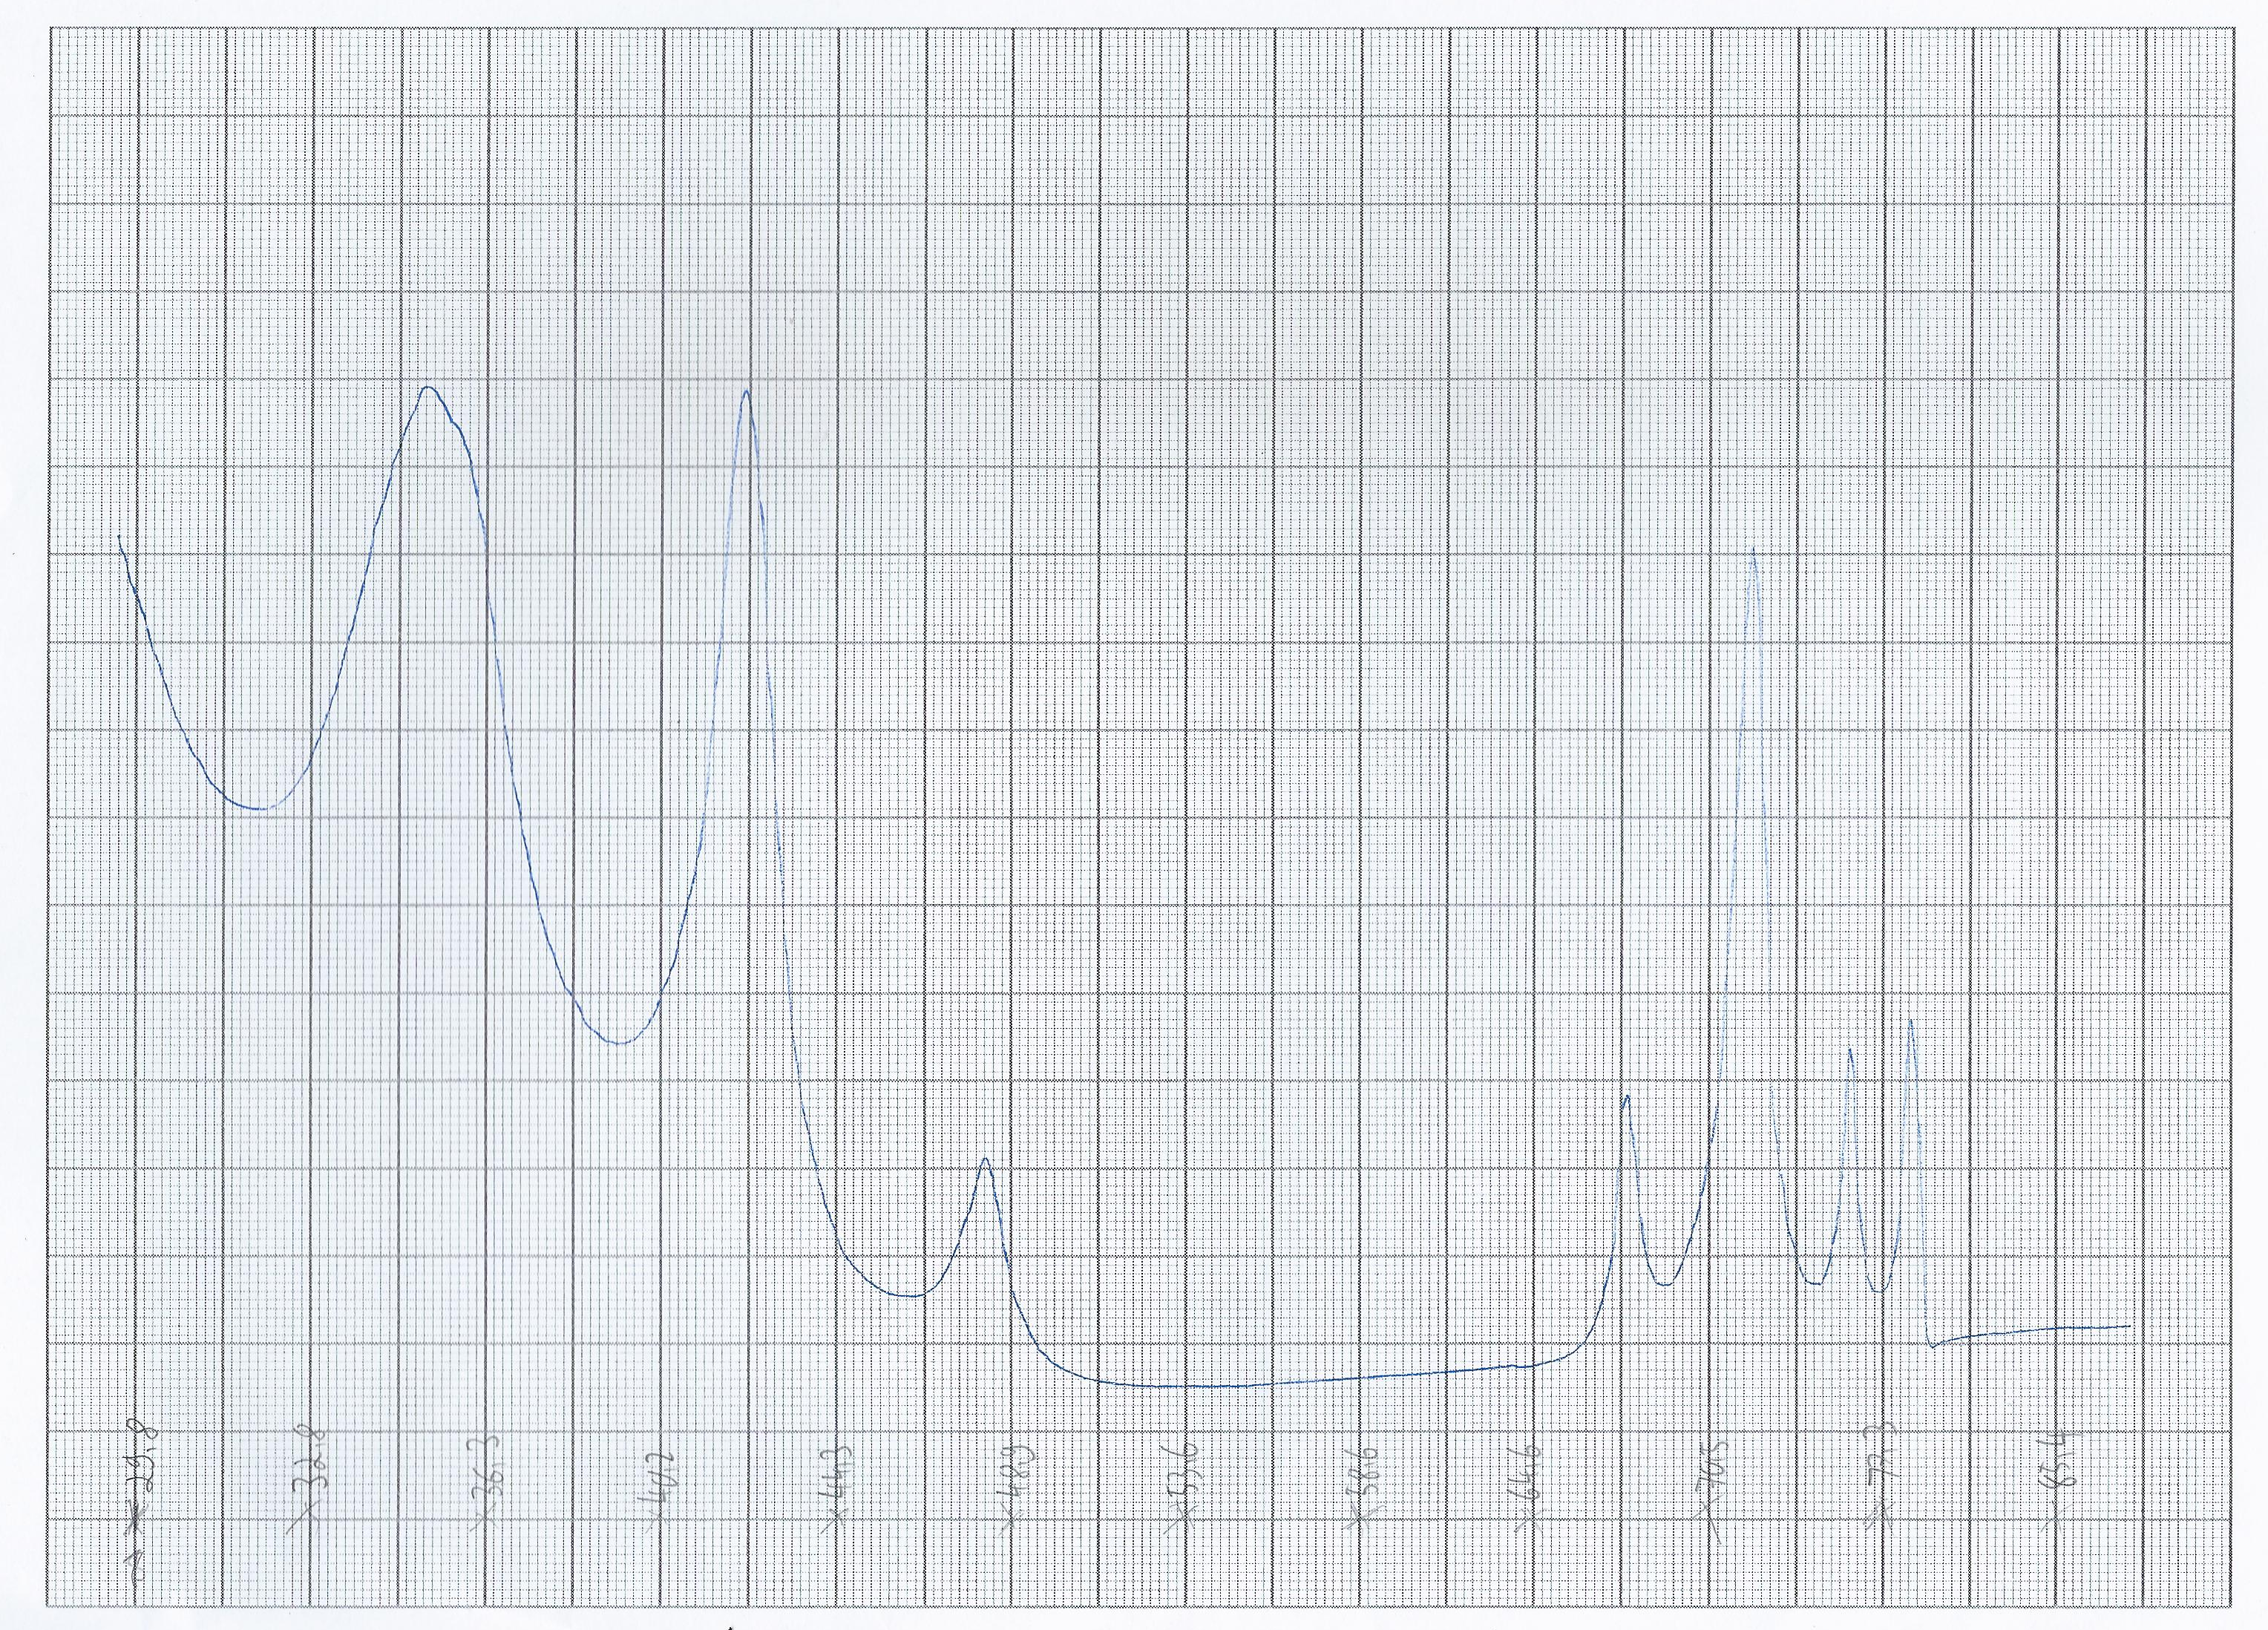
\includegraphics[angle=90, width=\textwidth]{aderlasskurve.png}[H]
  \caption{Aufgenommene Durchlasskurve der alternierenden Kette.}
  \label{fig:durchlass}
\end{figure}
\begin{table}
  \centering
  \caption{Exemplarisch abgelesene Frequenzen der Durchlasskurve der $LC$-Kette.}
  \label{tab:durchlass}
  \sisetup{table-format=1.2}
  \begin{tabular}{c c}
    \toprule
    {$LE [\si{\centi\metre}]$} & {$\nu [\si{\kilo\hertz}]$}\\
    \midrule
    \input{build/atabelle.tex}
    \bottomrule
  \end{tabular}
\end{table}
Die lineare Regression wird nun mit der Methode der kleinsten Quadrate mit Hilfe von SciPy durchgeführt.
Es ergeben sich die Parameter
\begin{align*}
  b &= \input{regres_b.tex}, \\
  m &= \input{regres_m.tex}.
\end{align*}
Die Grenzfrequenzen werden an der Durchlasskurve zu
\begin{align*}
  g_1 &= \SI{9}{\centi\metre} \\
  g_2 &= \SI{16.5}{\centi\metre}
\end{align*}
abgelesen.
Aus diesen Längenangaben und den in der linearen Regression bestimmten Parametern ergibt die Umrechnungsformel
\begin{equation}
  \nu = \mathrm{e}^{m g_i + b}
\end{equation}
die gesuchten Grenzfrequenzen.
Vergleicht man diese mit den aus Formel \ref{eqn:grenzfrequenzen} bestimmten Grenzfrequenzen, ergeben sich die Werte
\begin{align*}
  \nu_{1} &= \input{g1.tex}, \\
  \nu_{1, \text{theorie}} &= \input{g1_t.tex}, \\
  \nu_{2} &= \input{g2.tex}, \\
  \nu_{2, \text{theorie}} &= \input{g2_t.tex}.
\end{align*}


\subsection{Betrachtung der Dispersionsrelation}
Es wird nun die Dispersionsrelation, wie in der Durchführung beschrieben, betrachtet.
Dazu werden alle Frequenzen $\omega$ betrachtet, bei denen die Phasenverschiebung zwischen dem ersten und letzten $LC$-Glied ein Vielfaches von $\pi$ ist.
Aufgrund der Tatsache, dass die $LC$-Kette aus 14 alternierenden Gliedern besteht, folgt somit die jeweilige Phasenänderung pro Kettenglied $\theta$ zu $\frac{n \pi}{14}$.
Die gemessenen Werte sind in Tabelle \ref{tab:dispersion} angegeben.
\begin{table}
  \centering
  \caption{Bestimmung der Phasenverschebung pro Glied in Abhängigkeit der Frequenz.}
  \label{tab:dispersion}
  \sisetup{table-format=1.2}
  \begin{tabular}{c c c}
    \toprule
    {$\omega [\si{\hertz}]$} & {$\frac{\alpha}{\pi} $} & {$\frac{\theta}{\pi} $}\\
    \midrule
    \input{build/btabelle.tex}
    \bottomrule
  \end{tabular}
\end{table}
Hierbei beschreibt $\alpha$ die gemessene Phasenverschiebung zwischen dem ersten und letzten $LC$-Glied sowie $\theta$ die aus den obrigen Beobachtungen folgende Phasenverschiebung pro einzelnem Glied.
Bei der genaueren Auswertung der Messwerte ist aufgefallen, dass sich eine Unregelmäßigkeit zwischen dem siebten und achten Messwert ergeben hat.
Hieraus wird geschlussfolgert, dass der Messwert für die Phasenverschiebung $\alpha = 8 \pi$ versehentlich übersprungen wurde.
Dementsprechend ist für dieses $\alpha$ kein Messwert angegeben.
Mithilfe von Formel \ref{eqn:dispersion} können die Theoriekurven der Dispersionsrelation bestimmt werden.
Diese sind zusammen mit den gemessenen Werten in Abbildung \ref{fig:dispersion_fertig} dargestellt.
\begin{figure}
  \centering
  \includegraphics{dispersionsrelation.pdf}
  \caption{Gemessene sowie theoretisch bestimmte Dispersionsrelation der alternierenden Kette.}
  \label{fig:dispersion_fertig}
\end{figure}

\subsection{Bestimmung der Eigenfrequenzen}
Es werden nun, wie in der Durchführung beschrieben, die Eigenfrequenzen der offenen $LC$-Kette bestimmt.
Aufgrund der in Kapitel \ref{sec:verhalten} beschriebenen Eigenschaften der stehenden Wellen ergeben sich die Phasenverschiebungen von Anfang und Ende der LC-Kette zu Vielfachen von $\pi$, und die Phasenverschiebungen $\theta$ zu Vielfachen von $\frac{\pi}{14}$.
Die Phasengeschwindigkeit $v_{\text{Ph}}$ berechnet sich mit diesen Angaben nach \eqref{eqn:phase}.
Die gemessenen Werte sind in Tabelle \ref{tab:eigenfrequenzen} angegeben.
\begin{table}
  \centering
  \caption{Eigenfrequenzen sowie zugehörige Phasengeschwindigkeiten der $LC$-Kette.}
  \label{tab:eigenfrequenzen}
  \sisetup{table-format=1.2}
  \begin{tabular}{c c c}
    \toprule
    {$\omega [\si{\hertz}]$} & {$\frac{\theta}{\pi} $} & {$v_{\text{Ph}} [\si{\kilo\metre\per\second}] $}\\
    \midrule
    \input{build/ctabelle.tex}
    \bottomrule
  \end{tabular}
\end{table}
